\section{Lineare Gleichungssysteme - Direkte Löser I}

\subsection{Einleitung}

\begin{defi}{Lineares Gleichungssystem}
    Betrachten wir allgemein ein System von $m$ Gleichungen für $n$ Unbekannte, so erhalten wir:
    \[
        \begin{matrix}
            a_{11}x_1 & + & a_{12}x_2 & + & \cdots & + & a_{1n}x_n & = & b_1    \\
            a_{21}x_1 & + & a_{22}x_2 & + & \cdots & + & a_{2n}x_n & = & b_2    \\
            \vdots    &   &           &   &        &   &           &   & \vdots \\
            a_{m1}x_1 & + & a_{m2}x_2 & + & \cdots & + & a_{mn}x_n & = & b_m
        \end{matrix}
    \]
    Es gilt:
    \begin{itemize}
        \item Unbekannte dürfen nur linear auftreten,
        \item $a_{ij} \in \R$ gegebene Koeffizienten,
        \item $b_i \in \R$ gegebene rechte Seite,
        \item $x_j \in \R$ gesuchte Unbekannte
    \end{itemize}

    Zur Abkürzung benutzt man die Matrix-Vektor-Schreibweise
    \[
        Ax = b
    \]
    mit Systemmatrix
    \[
        A =
        \begin{pmatrix}
            a_{11} & \cdots & a_{1n} \\
            \vdots &        & \vdots \\
            a_{m1} & \cdots & a_{mn}
        \end{pmatrix}
        \in \R^{m \times n},
    \]
    rechter Seite
    \[
        b =
        \begin{pmatrix}
            b_1    \\
            \vdots \\
            b_m
        \end{pmatrix}
        \in \R^{m},
    \]
    Vektor der Unbekannten
    \[
        x =
        \begin{pmatrix}
            x_1    \\
            \vdots \\
            x_n
        \end{pmatrix}
        \in \R^{n}
    \]
    und Matrix-Vektor-Produkt
    \[
        Ax =
        \begin{pmatrix}
            a_{11} & \cdots & a_{1n} \\
            \vdots &        & \vdots \\
            a_{m1} & \cdots & a_{mn}
        \end{pmatrix}
        \begin{pmatrix}
            x_1    \\
            \vdots \\
            x_n
        \end{pmatrix}
        =
        \begin{pmatrix}
            a_{11}x_1 & + & a_{12}x_2 & + & \cdots & + & a_{1n}x_n \\
            \vdots    &   &           &   &        &   & \vdots    \\
            a_{m1}x_1 & + & a_{m2}x_2 & + & \cdots & + & a_{mn}x_n
        \end{pmatrix}
    \]
\end{defi}

\begin{bonus}{Lösbarkeit von linearen Gleichungssystemen}
    Sei ein lineares Gleichungssystem mit $A \in \R^{m \times n}$, $b \in \R^{m}$ und $x \in \R^{n}$ gegeben.

    Dann gilt:
    \begin{itemize}
        \item $m \neq n$ $\implies$ (in der Regel) entweder keine Lösung oder unendlich viele,
        \item $m = n$ $\implies$ eindeutig lösbar, falls $A$ regulär\footnote{$A \in \R^{n\times n}$ heißt \emph{regulär}, falls $\det(A) \neq 0$ bzw. \emph{singulär}, falls $\det(A) = 0$.} ist.
    \end{itemize}
\end{bonus}

\begin{bonus}{Wiederholung Matrizen}
    Es gilt:
    \begin{itemize}
        \item $\det(A) \neq 0$ $\iff$ Spalten $s_j = \begin{pmatrix} a_{1j} \\ \vdots \\ a_{nj} \end{pmatrix}$, $j = 1, \ldots, n$ sind linear unabhängig.
        \item $\det(A) \neq 0$ $\iff$ Zeilen $z_i = \begin{pmatrix} a_{i1} & \cdots & a_{in} \end{pmatrix}$, $i = 1, \ldots, n$ sind linear unabhängig.
        \item $A \in \R^{n \times n}$ regulär $\iff$ $\rang(A) = n$
        \item $A \in \R^{n \times n}$ singulär $\iff$ $\rang(A) < n$
        \item $A \in \R^{m \times n}$ definiert eine lineare Abbildung $\R^n \to \R^m$ durch $x \to Ax$.
        \item Jede lineare Abbildung $\R^n \to \R^m$ ist als Matrix darstellbar.
        \item Matrizenmultiplikation ist nur bei passender Dimension möglich.
        \item In der Regel ist Matrizenmultiplikation nicht kommutativ (also $AB \neq BA$).
        \item $(AB)^T = B^TA^T$
        \item $A, B \in \R^{n \times n} \implies \det(AB) = \det(A) \det(B) \implies$ sind $A$, $B$ regulär, dann auch $AB$
        \item Ist $A \in \R^{n \times n}$ regulär, so existiert die Inverse $A^{-1} \in \R^{n \times n}$ mit
              \[
                  A^{-1}A = AA^{-1} = I =
                  \begin{pmatrix}
                      1 &        &   \\
                        & \ddots &   \\
                        &        & 1
                  \end{pmatrix}
              \]
        \item für $A, B$ regulär ist $(AB)^{-1} = B^{-1}A^{-1}$
    \end{itemize}
\end{bonus}

\begin{defi}{Matrixnorm}
    Ist $\norm{\cdot}$ eine Norm auf $\R^n$, $A \in \R^{n \times n}$, dann definiert
    \[
        \norm{A} := \sup_{x \neq 0} \frac{\norm{Ax}}{\norm{x}} = \max_{\norm{x} = 1} \norm{Ax}
    \]
    eine \emph{Matrixnorm} auf $\R^{n \times n}$.

    Eine Matrixnorm erfüllt analog zur Vektornorm die folgenden Bedingungen:
    \begin{enumerate}
        \item $\norm{A} = 0 \iff x = 0$ (Definitheit)
        \item $\norm{\alpha A} = \alpha \norm{A} \quad \forall A \in \R^{n \times n}, \forall \alpha \in \R$ (absolute Homogenität)
        \item $\norm{A + B} \leq \norm{A} + \norm{B} \quad \forall A, B \in \R^{n \times n}$ (Subadditivität oder Dreiecksungleichung)
    \end{enumerate}

    Eine Matrixnorm hängt von der benutzten Vektornorm ab und heißt deshalb die von der Vektornorm \emph{induzierte Matrixnorm}.

    Eine Vektornorm und die induzierte Matrixnorm sind kompatibel, d.h.
    \[
        \norm{Ax} \leq \norm{A} \norm{x}
    \]

    Für induzierte Matrixnormen gilt
    \[
        \norm{AB} \leq \norm{A} \norm{B}
    \]

    Auf $\R^{n \times n}$ sind alle Matrixnormen äquivalent.
\end{defi}

\begin{defi}{Spektralnorm}
    \begin{wrapfigure}{r}{0.4\textwidth}
        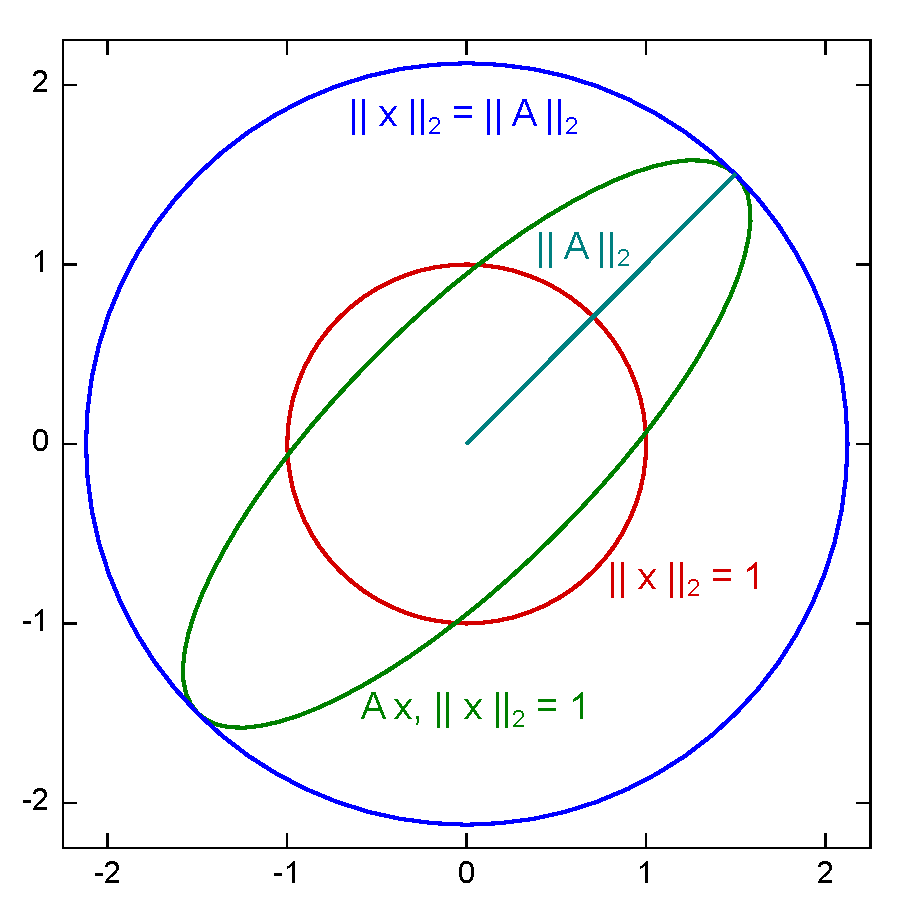
\includegraphics[width=.35\textwidth]{includes/figures/defi_spektralnorm.pdf}
    \end{wrapfigure}
    %
    Für $\| \cdot \|_2$ erhält man als induzierte Matrixnorm die \emph{Spektralnorm}
    \[
        \| A \|_2 = \sqrt{\rho (A^TA)}
    \]
    wobei der \emph{Spektralradius} $\rho(B)$ der betragsgrößte Eigenwert von $B$ ist.

    Anschaulich entspricht die Spektralnorm damit dem größtmöglichen Streckungsfaktor, der durch die Anwendung der Matrix auf einen Vektor der Länge Eins entsteht.

    Eine äquivalente Definition der Spektralnorm ist der Radius der kleinsten Sphäre, die den Einheitskreis nach Transformation durch die Matrix umfasst.
\end{defi}

\begin{defi}{Zeilensummennorm}
    \begin{wrapfigure}{r}{0.4\textwidth}
        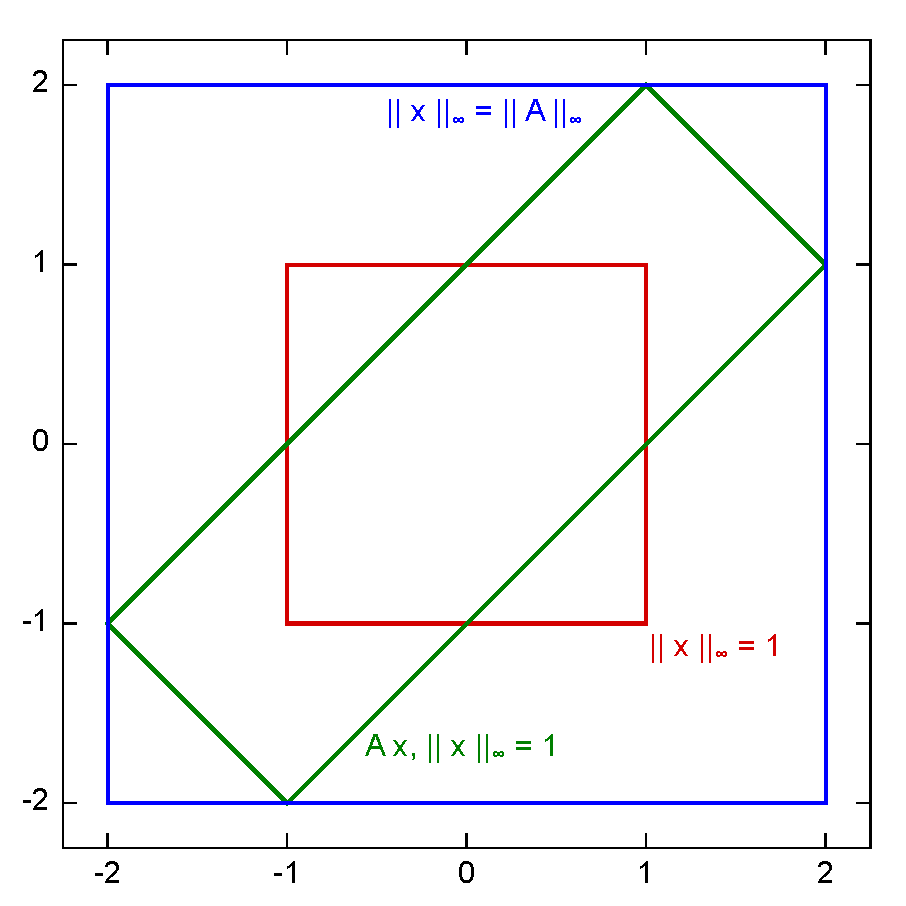
\includegraphics[width=.35\textwidth]{includes/figures/defi_zeilensummennorm.pdf}
    \end{wrapfigure}
    %
    Für $\| \cdot \|_\infty$ erhält man als induzierte Matrixnorm die \emph{Zeilensummennorm}
    \[
        \| A \|_\infty = \max_{i = 1, \ldots, n} \sum_{j = 1}^{n} | a_{ij} |
    \]

    Anschaulich entspricht die Zeilensummennorm dem größtmöglichen Streckungsfaktor, der durch die Anwendung der Matrix auf einen Vektor mit \emph{betragsmaximalen Eintrag Eins} entsteht.

    Für die Zeilensummennorm gilt die namensgebende Darstellung:
    \[
        \| A \|_\infty = \max_{\| x \|_\infty = 1} \| Ax \|_\infty = \max_{\| x \|_\infty = 1} \max_{i=1, \ldots ,n} \left| \sum_{j=1}^n a_{ij} x_j \right| = \max_{i=1, \ldots ,n} \max_{\| x \|_\infty = 1} \left| \sum_{j=1}^n a_{ij} x_j \right| = \max_{i=1, \ldots ,n}{\sum_{j=1}^n | a_{ij} |}
    \]\
    Hierbei wurde genutzt, dass die Summe innerhalb der Betragsstriche für festes $i$ genau dann maximal wird, wenn $x_j = \sign(a_{ij})$ für alle $j$ ist.

    Die Berechnung der Zeilensummennorm erfolgt also durch die Ermittlung der Betragssumme jeder Zeile und dann durch Auswahl des Maximums dieser Werte.
\end{defi}

\begin{defi}{Spaltensummennorm}
    \begin{wrapfigure}{r}{0.4\textwidth}
        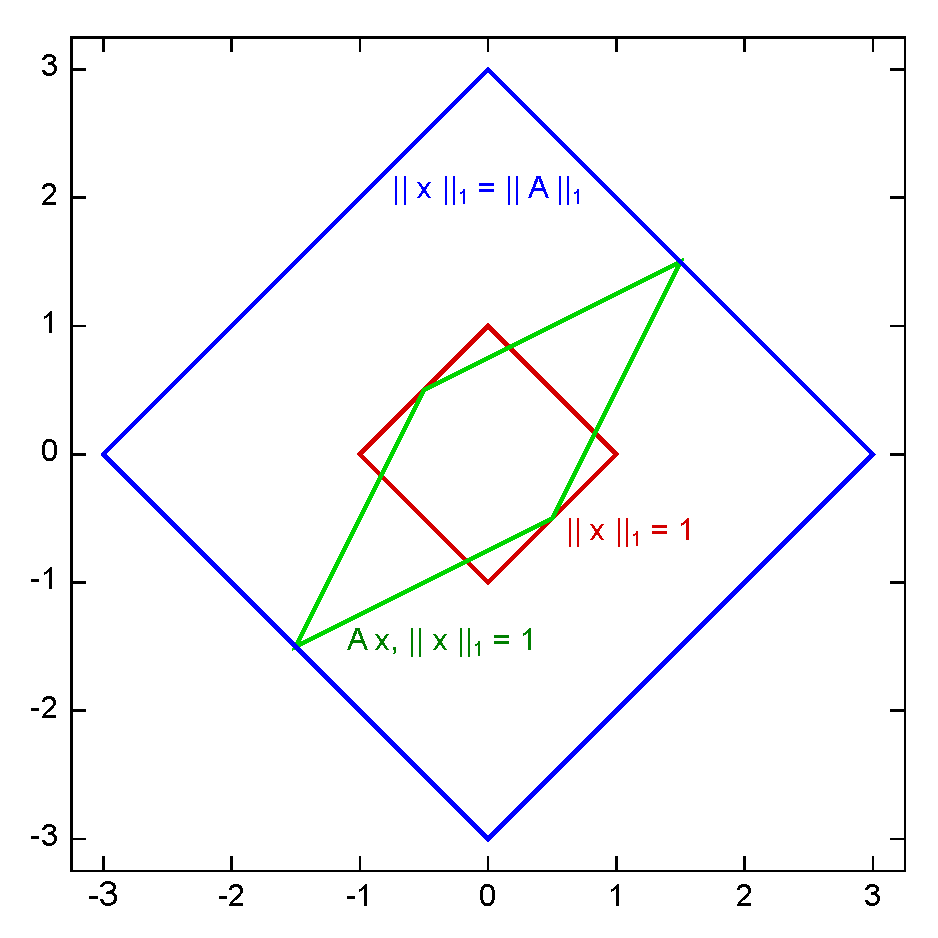
\includegraphics[width=.35\textwidth]{includes/figures/defi_spaltensummennorm.pdf}
    \end{wrapfigure}
    %
    Für $\| \cdot \|_1$ erhält man als induzierte Matrixnorm die \emph{Spaltensummennorm}
    \[
        \| A \|_\infty = \max_{j = 1, \ldots, n} \sum_{i = 1}^{n} | a_{ij} |
    \]

    Anschaulich entspricht die Spaltensummennorm dem größtmöglichen Streckungsfaktor, der durch die Anwendung der Matrix auf einen Vektor mit \emph{Betragssumme Eins} entsteht.

    Für die Spaltensummennorm gilt die namensgebende Darstellung:
    \[
        \|A\|_{1}=\max _{\|x\|_{1}=1}\|Ax\|_{1}=\max _{\|x\|_{1}=1}\sum _{i=1}^{n}\left|\sum _{j=1}^{n}a_{ij}x_{j}\right|=\max _{j=1,\ldots ,n}\sum _{i=1}^{n}|a_{ij}|
    \]
    Hierbei wurde genutzt, dass die Summe innerhalb der Betragsstriche für festes $i$ für einen der Einheitsvektoren $x = \pm e_j$ mit $j = 1, \ldots ,n$ maximal wird.

    Die Berechnung der Spaltensummennorm erfolgt also durch die Ermittlung der Betragssumme jeder Spalte und dann durch Auswahl des Maximums dieser Werte.
\end{defi}

\begin{defi}{Frobeniusnorm}
    Die \emph{Frobeniusnorm}
    \[
        \| A \|_F = \sqrt{\spur(A^TA)}, \quad \spur(C) = \sum_{i=1}^{n} \sum_{j=1}^{n} c_{ij}^2
    \]
    ist \emph{nicht induziert}, erfüllt aber
    \[
        \| AB \|_F \leq \| A \|_F \cdot \| B \|_F
    \]
    und ist wegen
    \[
        \| Ax \|_2 \leq \| A \|_F \cdot \| x \|_F \quad \forall x
    \]
    mit der Vektornorm $\| \cdot \|_2$ verträglich.

    $\| A \|_F$ ist eine obere Schranke für $\| A \|_2$, aber deutlich einfacher zu berechnen.

    Die Frobeniusnorm entspricht damit der euklidischen Norm eines Vektors der Länge $m \cdot n$, in dem alle Einträge der Matrix untereinander notiert sind.
\end{defi}

\subsection{Gaußelimination}

\begin{defi}{Gaußelimination}
    Die \emph{Gaußelimination} ist ein wichtiges Verfahren zum Lösen von linearen Gleichungssystemen und beruht darauf, dass Äquivalenztransformationen zwar das Gleichungssystem ändern, aber die Lösung erhalten.

    Dies erlaubt es, jedes eindeutig lösbare Gleichungssystem auf Dreiecksgestalt zu bringen, an der die Lösung durch sukzessive Elimination der Unbekannten leicht ermittelt oder die Lösungsmenge abgelesen werden kann.

    Die Anzahl der benötigten Operationen ist bei einer $n \times n$-Matrix von der Größenordnung $n^3$.

    In seiner Grundform ist der Algorithmus aus numerischer Sicht anfällig für Rundungsfehler, aber mit kleinen Modifikationen (Pivotisierung) stellt er für allgemeine lineare Gleichungssysteme das Standardlösungsverfahren dar.
\end{defi}

\begin{algo}{Gaußelimination}
    Ein lineares Gleichungssystem $Ax = b$ mit $n$ Gleichungen und $n$ Unbekannten \\
    $x = \begin{pmatrix} x_1 & x_2 & \cdots & x_n \end{pmatrix}^T$ und rechter Seite $b = \begin{pmatrix} b_1 & b_2 & \cdots & b_n \end{pmatrix}^T$ hat die Form:
    \[
        \begin{matrix}
            a_{11} x_1 & + & a_{12} x_2 & + & \cdots & + & a_{1n} x_n & = & b_1    \\
            a_{21} x_1 & + & a_{22} x_2 & + & \cdots & + & a_{2n} x_n & = & b_2    \\
            \vdots     & + & \vdots     & + & \ddots & + & \vdots     & = & \vdots \\
            a_{n1} x_1 & + & a_{n2} x_2 & + & \cdots & + & a_{nn} x_n & = & b_n
        \end{matrix}
    \]

    Der Algorithmus zur Berechnung der Variablen $x_i$ lässt sich in zwei Etappen einteilen:
    \begin{enumerate}
        \item Vorwärtselimination,
        \item Rückwärtseinsetzen (Rücksubstitution).
    \end{enumerate}

    Im ersten Schritt wird das Gleichungssystem auf Dreiecksgestalt gebracht.
    Dreiecksgestalt heißt, dass pro Zeile mindestens eine Variable weniger auftritt, also mindestens eine Variable \emph{eliminiert} wird.
    Wir erhalten:
    \[
        \begin{matrix}
            \tilde{a}_{11} x_1 & + & \tilde{a}_{12} x_2 & + & \cdots & + & \tilde{a}_{1n} x_n & = & \tilde{b}_1 \\
                               &   & \tilde{a}_{22} x_2 & + & \cdots & + & \tilde{a}_{2n} x_n & = & \tilde{b}_2 \\
                               &   &                    &   & \ddots & + & \vdots             & = & \vdots      \\
                               &   &                    &   &        &   & \tilde{a}_{nn} x_n & = & \tilde{b}_n
        \end{matrix}
    \]

    Zum Erreichen der Dreiecksgestalt werden elementare Zeilenumformungen benutzt, mit Hilfe derer das Gleichungssystem in ein neues transformiert wird, welches aber dieselbe Lösungsmenge besitzt.

    Ausreichend sind zwei Arten von elementaren Zeilenumformungen:
    \begin{enumerate}
        \item Eine Zeile oder das Vielfache einer Zeile zu einer anderen Zeile addieren.
        \item Zwei Zeilen vertauschen.
    \end{enumerate}

    Das Verfahren besteht dann darin, angefangen in der ersten Spalte mit Umformungen der ersten Art durch geschicktes Dazuaddieren der ersten Zeile alle Einträge bis auf den ersten zu Null zu machen.
    Dies wird dann in der so modifizierten zweiten Spalte fortgesetzt, wobei diesmal Vielfache der zweiten Zeile zu den folgenden Zeilen addiert werden und so weiter.

    Dieser Schritt funktioniert nur, wenn das Diagonalelement der aktuellen Spalte nicht Null ist.
    In so einem Fall ist die zweite Art der Zeilenumformung nötig, da durch eine Zeilenvertauschung ein Nichtnulleintrag auf der Diagonale erzeugt werden kann.
    Mit Hilfe dieser beiden Arten von Umformungen ist es möglich, jedes lineare Gleichungssystem auf Dreiecksgestalt zu bringen.

    Im zweiten Schritt des Verfahrens, dem Rückwärtseinsetzen, werden ausgehend von der letzten Zeile, in der nur noch eine Variable auftaucht, die Variablen ausgerechnet und in die darüberliegende Zeile eingesetzt.
\end{algo}

\begin{example}{Gaußelimination}
    TO DO
\end{example}

\subsection{LU-Zerlegung}

\begin{defi}{Frobeniusmatrix}
    Eine Matrix ist eine \emph{Frobeniusmatrix}, wenn sie die folgenden drei Eigenschaften aufweist:
    \begin{itemize}
        \item auf der Hauptdiagonale stehen nur Einsen,
        \item in höchstens einer Spalte stehen unter der Hauptdiagonale beliebige Einträge,
        \item alle anderen Einträge sind Null.
    \end{itemize}

    Frobeniusmatrizen haben stets eine Determinante vom Wert 1 und sind somit invertierbar.
    Ihre inverse Matrix wird gebildet, indem das Vorzeichen aller Einträge außerhalb der Hauptdiagonalen gewechselt wird.

    Frobeniusmatrizen treten bei der Beschreibung des Gaußschen Eliminationsverfahrens als Darstellungsmatrizen der Gaußelimination auf.

    Wird eine Matrix von links mit einer Frobeniusmatrix multipliziert, dann wird ein skalares Vielfaches einer bestimmten Zeile zu einer oder mehreren darunter liegenden Zeilen addiert.
    Dies entspricht einer der Elementaroperationen des Gaußschen Eliminationsverfahrens (neben der Operation der Vertauschung von Zeilen und der Multiplikation einer Zeile mit einem skalaren Vielfachen).
\end{defi}

\begin{example}{Frobeniusmatrix}
    Sei zunächst
    \[
        A = \begin{pmatrix}
            a_{11} & a_{12} \\
            a_{21} & a_{22}
        \end{pmatrix}
        \quad
        a_{11} \neq 0
    \]

    $a_{21}$ wird eliminiert, indem von der zweiten Zeile $\frac{a_{21}}{a_{11}}$-mal Zeile 1 abgezogen wird.

    Das kann als Matrixmultiplikation geschrieben werden.
    Es folgt mit
    \[
        F = \begin{pmatrix}
            1                      & 0 \\
            -\frac{a_{21}}{a_{11}} & 1
        \end{pmatrix}
        = \begin{pmatrix}
            1       & 0 \\
            -l_{21} & 1
        \end{pmatrix}:
    \]
    \[
        FA =
        \begin{pmatrix}
            1                      & 0 \\
            -\frac{a_{21}}{a_{11}} & 1
        \end{pmatrix}
        \begin{pmatrix}
            a_{11} & a_{12} \\
            a_{21} & a_{22}
        \end{pmatrix}
        =
        \begin{pmatrix}
            a_{11}                                 & a_{12}                                 \\
            -\frac{a_{21}}{a_{11}} a_{11} + a_{21} & -\frac{a_{21}}{a_{11}} a_{12} + a_{22}
        \end{pmatrix}
        =
        \begin{pmatrix}
            a_{11} & a_{12}                                \\
            0      & a_{22} - \frac{a_{21}}{a_{11}} a_{12}
        \end{pmatrix}
    \]

    Analog folgt für die Elimination der $k$-ten Spalte $A^{(k-1)} \to A^{(k)}$ im allgemeinen Fall:
    \[
        A^{(k)} = F_kA^{(k-1)}, \quad F_k =
        \begin{pmatrix}
            1 &        &           &   &            \\
              & \ddots &           &   &            \\
              &        & 1         &   &            \\
              &        & -l_{k+1k} & 1 &            \\
              &        & \vdots    &   & \ddots &   \\
              &        & -l_{nk}   &   &        & 1
        \end{pmatrix}
        \in \R^{n \times n}
    \]

    mit
    \[
        l_{ik} = \frac{a^{(k-1)}_{ik}}{a^{(k-1)}_{kk}}
    \]
\end{example}

\begin{bonus}{LU-Zerlegung (Motivation)}
    Die Gaußelimination liefert für ein lineares Gleichungssystem $Ax = b$
    \[
        A \to A^{(1)} \to \ldots \to A^{(n-1)} = U
    \]
    \[
        b \to b^{(1)} \to \ldots \to b^{(n-1)}
    \]

    Sie liefert für ein zweites lineares Gleichungssystem $Ax' = b'$ für identisches $A$ ein gleiches $U$.

    Diesen doppelten Aufwand kann man sich sparen mithilfe der \emph{LU-Zerlegung} sparen.
\end{bonus}

\begin{defi}{LU-Zerlegung}
    Sind alle $a^{(k-1)}_{kk} \neq 0$, so erzeugt die Gaußelimination eine \emph{LU-Zerlegung}
    \[
        A = LU
    \]
    von $A$, wobei $L$ eine unter Dreiecksmatrix mit Diagonale $1$ und $U$ eine obere Dreiecksmatrix ist.

    Hat man für $A$ einmal eine Gaußelimination durchgeführt, so kennt man $L$ und $U$.

    $LUx = b$ ist sehr leicht zu lösen:
    \begin{enumerate}
        \item löse $Ly = b$, dann $Ux = y$
        \item $x$ ist die gesuchte Lösung, da $b = Ly = LUx = Ax$
        \item $Ux = y$ kann durch Rückwärtseinsetzen gelöst werden, da $U$ obere Dreiecksmatrix
        \item $Ly = b$ kann durch Vorwärtseinsetzen gelöst werden, da $L$ untere Dreiecksmatrix
    \end{enumerate}

    Der Aufwand der LU-Zerlegung ist wie folgt:
    \begin{itemize}
        \item $Ax = b$ mit Gaußelimination $\approx \frac{2}{3} n^3$,
        \item $L$, $U$ bestimmen mit Gaußelimination $\approx \frac{2}{3} n^3$,
        \item $LUx = b$ lösen $\approx 2n^2$
        \item $\implies$ ist $L$, $U$ bekannt, so ist die Lösung für verschiedene $b$ \enquote{günstig} zu erhalten
    \end{itemize}

    Da wir wissen, dass auf der Hauptdiagonalen von $L$ $1$en sind, brauchen diese nicht explizit gespeichert zu werden.
    Der Rest von $L$, $U$ \enquote{passt} in den Speicherbereich von $A$.
    $A$ selbst brauchen wir dann nicht mehr, da $Ax = b \iff LUx = b$ ist.
\end{defi}

\begin{example}{LU-Zerlegung}
    TODO
\end{example}

\begin{defi}{Permutationsmatrix}
    Eine \emph{Permutationsmatrix} ist eine quadratische Matrix, bei der genau ein Eintrag pro Zeile und Spalte gleich $1$ ist und alle anderen Einträge gleich $0$ sind.

    Der Zeilentausch der Gaußelimination der Zeilen $i$ und $j$ kann dargestellt werden durch die Identitätsmatrix $I$ mit den Zeilen $i$ und $j$ vertauscht.

    $PA$ tauscht die Zeilen $i$ und $j$, $AP$ tauscht die Spalten $i$ und $j$.

    Für Permutationen gilt:
    \begin{itemize}
        \item $P = P^T$
        \item $PP = I$
        \item $P = P^{-1}$
    \end{itemize}
\end{defi}

\begin{bonus}{LU-Zerlegung für beliebige reguläre Matrizen (Idee)}
    Sei $A$ regulär, $A^{(k-1)} = F_{k-1} \ldots F_1 A$ mit Hilfe der Gaußelimination erzeugt und $a^{(k-1)}_{kk} = 0$.

    Dann gibt es in der $k$-ten Spalte unterhalb der Diagonalen immer mindestens ein Element $a^{(k-1)}_{ik}$ mit $a^{(k-1)}_{ik} \neq 0$ und $i > k$, d.h. ein erfolgreicher Zeilentausch ist immer möglich.

    Bevor $F_k$ die $k$-te Spalte eliminiert, muss eventuell getauscht werden.
    Damit erhalten wir:
    \[
        U = F_{n-1} P_{n-1} \cdot \ldots \cdot F_1 P_1 A
    \]
    wobei $U$ eine obere Dreiecksmatrix ist und $P_i$ Permutationsmatrizen oder $P_i = I$\footnote{was auch eine Permutation ist.}.

    Es gilt:
    \[
        A = \tilde{L} U \quad \iff \quad U = \tilde{L}^{-1} A, \quad \tilde{L} = (F_{n-1} P_{n-1} \cdot \ldots \cdot F_1 P_1)^{-1}
    \]

    $\tilde{L}$ ist in der Regel \emph{keine} untere Dreiecksmatrix.

    Wir erhalten ein $L$ in entsprechender Dreiecksgestalt durch:
    \[
        PA = LU \quad \iff \quad U = L^{-1} PA, \quad P = P_{n-1} \cdot \ldots \cdot P_1
    \]
\end{bonus}

\begin{defi}{LU-Zerlegung für beliebige reguläre Matrizen}
    Sei $A \in \R^{n \times n}$ regulär, so gibt es Permutationen $P_k$, $k = 1, \ldots, n-1$ so, dass mit $P = P_1 \cdot \ldots \cdot P_n$ gilt:
    \[
        PA = LU
    \]
    wobei $L$ eine untere Dreiecksmatrix mit $\diagonal(L) = 1$ und $U$ eine obere Dreiecksmatrix ist.

    Tauscht man vorab die Zeilen in $A$ entsprechend $P$, so sind alle $a^{k-1}_{kk} \neq 0$, d.h. $PA = LU$.

    Die Permutation $P$ ist nicht vorher bekannt, sondern ergibt sich erst während der LU-Zerlegung.
\end{defi}


\begin{defi}{LU-Zerlegung für beliebige reguläre Matrizen (Praxis)}
    Es gilt:
    \[
        Ax = b \quad \iff \quad PAx = Pb \quad \iff \quad LUx = Pb
    \]

    Implementiert werden drei Routinen:
    \begin{enumerate}
        \item LU-Zerlegung mit Permutation durch Gaußelimination liefert $L$, $U$ und $P$
        \item löse $Ly = Pb$ durch Vorwärtseinsetzen
        \item löse $Ux = y$ durch Rückwärtseinsetzen
    \end{enumerate}

    Es gilt $P = P_{n-1} \cdot \ldots \cdot P_1$ wobei $P_k$ die $k$-te Zeile mit einer Zeile $j_k > k$ vertauscht.

    Deshalb können alle $P_k$ in einem einzigen ganzzahligen Vektor
    \[
        p = \begin{pmatrix}
            j_1    \\
            j_2    \\
            \vdots \\
            j_{n-1}
        \end{pmatrix}
    \]
    abgespeichert werden.

    $L$ wird im freiwerdenden Teil von $A$ gespeichert.
    Insgesamt ergibt sich für einen Eliminationsschritt:
    \begin{itemize}
        \item suche $j_k$
        \item tausche komplette Zeile im 2D-Array, in dem ursprünglich $A$ abgelegt ist
        \item eliminiere $k$-te Spalte wie üblich
    \end{itemize}
\end{defi}

\subsection{Cholesky-Zerlegung}

\begin{defi}{Cholesky-Zerlegung}
    Sei $A \in \R^{n \times n}$ symmetrisch positiv definit.
    Dann kann $A$ wie folgt zerlegt werden:
    \begin{itemize}
        \item \emph{rationale Cholesky-Zerlegung}
              \[
                  A = \tilde{L} D \tilde{L}^T
              \]
              \begin{itemize}
                  \item $\tilde{L}$ untere Dreiecksmatrix mit $\diagonal(L) = 1$
                  \item $D$ Diagonalmatrix mit positiven Diagonalelementen
              \end{itemize}
        \item \emph{Cholesky-Zerlegung}
              \[
                  A = LL^T
              \]
              \begin{itemize}
                  \item $L$ untere Dreiecksmatrix
              \end{itemize}
    \end{itemize}

    Die Cholesky-Zerlegung basiert auf der Gaußelimination mit zusätzlicher Multiplikation mit $F_k^T$, was zunächst einen höheren Aufwand erwarten lässt.
    $F_k^T$ eliminiert aber nur die entsprechende Zeile und hat sonst keinen Einfluss, d. h. es ist nichts weiter zu tun als $0$ in die Matrix einzutragen.

    Alle $A^{(k)}$ sind symmetrisch, weshalb nur eine Hälfte der Koeffizienten berechnet werden muss.
\end{defi}

\begin{defi}{Cholesky-Zerlegung (Praxis)}
    Für die praktische Durchführung der Cholesky-Zerlegung wird in der Regel eine andere Form benutzt, die gar nicht an Gauß erinnert.

    Sei $A \in \R^{n \times n}$ symmetrisch positiv definit mit $A = LL^T$,
    \[
        L = \begin{pmatrix}
            l_{11} &        &        &        \\
            l_{21} & l_{22} &        &        \\
            \vdots & \vdots & \ddots &        \\
            l_{n1} & l_{n2} & \cdots & l_{nn}
        \end{pmatrix}
    \]

    Der $k$-te Schritt des Cholesky-Verfahrens besteht aus:
    \begin{enumerate}
        \item Berechne $k$-te Spalte:
              \begin{itemize}
                  \item
                        \[
                            l_{kk} = \sqrt{a^{(k)}_{kk}}
                        \]
                  \item
                        \[
                            l_{ik} = \frac{a^{(k)}_{ik}}{l_{kk}}
                        \]
                        \begin{itemize}
                            \item $i = k + 1, \ldots, n$
                        \end{itemize}
              \end{itemize}
        \item Berechne $A^{(k+1)}$:
              \begin{itemize}
                  \item
                        \[
                            a^{(k+1)}_{ij} = a^{(k)}_{ij} - l_{ik} l_{jk}
                        \]
                        \begin{itemize}
                            \item $i = k + 1, \ldots, n$
                            \item $j = k + 1, \ldots, i$
                        \end{itemize}
              \end{itemize}
    \end{enumerate}

    Ist $A = LL^T$ bekannt, so verfährt man zur Lösung von $Ax = b$ wie üblich:
    \[
        Ax = b \quad \iff \quad LL^Tx = b \quad \iff \quad Ly = b, L^Tx = y
    \]
    \begin{itemize}
        \item $Ly = b$ wird durch Vorwärtseinsetzen gelöst.
        \item $L^Tx = y$ wird durch Rückwärtseinsetzen gelöst.
    \end{itemize}
\end{defi}

\begin{example}{Cholesky-Zerlegung}
    TODO
\end{example}